\chapter{Przeprowadzone testy}
\label{ch:tests}
W tym rozdziale omówione zostało przeprowadzenie testów zaimplementowanych algorytmów.

Należy zaznaczyć, że wspomniane w tym rozdziale testy powinny być rozumiane jako eksperymenty przeprowadzenia symulacji planowania tras dla wielu robotów mobilnych, mające na celu zebranie statystycznych danych o przebiegu i rezultatach tych symulacji. Zatem już z założenia część tych testów może zakończyć się niepowodzeniem.
Nie należy mylić tego z automatycznymi testami poprawności wykonywanymi podczas rozwijania aplikacji w ramach podejścia TDD ({\it Test-Driven Development}), które zostały opisane w jednym z poprzednich rozdziałów (por. \ref{ch:junit-tdd}).

W ramach testów metod planowania tras wykonano pomiary skuteczności oraz wydajności w różnych środowiskach. 
Środowiska te były generowane w sposób losowy, dlatego z obszernych pomiarów zbierano statystyczne wyniki będące wartością średnią mierzonych wskaźników.

Wśród testowanych algorytmów znalazły się:
\begin{itemize}
	\item Algorytm A* bez rozwiązywania kolizji (por. \ref{ch:alg-single-astar}),
	\item LRA* - Local-Repair A* (por. \ref{ch:alg-collision-avoid}),
	\item WHCA*1 - Windowed Hierarchical Cooperative A* bez dynamicznego przydzielania priorytetów, ze stałym oknem czasowym (por. \ref{ch:alg-whca}),
	\item WHCA*2 - Windowed Hierarchical Cooperative A* z dynamicznym przydziałem priorytetów, ze stałym oknem czasowym (por. \ref{ch:alg-priorities-allocation}),
	\item WHCA*3 - Windowed Hierarchical Cooperative A* z dynamicznym przydziałem priorytetów oraz skalowaniem okna czasowego (por. \ref{ch:alg-priorities-allocation}).
\end{itemize}

Mierzonymi wskaźnikami były:
\begin{itemize}
	\item liczba wystąpień pomyślnego, bezkolizyjnego doprowadzenia wszystkich robotów do ich celów oraz "skuteczność" rozumiana jako iloraz liczby udanych planowań do liczby wszystkich symulacji,
	\item liczba kroków symulacji (minimalny czas wykonywania akcji w rzeczywistym środowisku do momentu doprowadzenia wszystkich robotów do celu),
	\item złożoność obliczeniowa planowania (czas wykonywania obliczeń dla samego wyznaczania tras w ciągu całej symulacji).
\end{itemize}

\section{Automatyczne zarządzanie symulacjami}
Na potrzeby wszystkich testów, których wyniki zamieszczono w rozdziale \ref{ch:tests}, przeprowadzono razem $76\ 800$ automatycznie zarządzanych symulacji ruchu robotów. Wykonano to dla różnych metod planowania, z różnymi parametrami i na różnych mapach oraz układach robotów.

Do automatycznego wykonywania symulacji wykorzystano bibliotekę {\it jUnit}. Choć w standardowym zastosowaniu służy ona do wykonywania automatycznych testów jednostkowych sprawdzających poprawność pojedynczych komponentów aplikacji, to jednak wykorzystano ją tutaj ze względu na możliwość uruchomienia istniejących fragmentów aplikacji w innym trybie.
Pozwala to na wykonanie serii symulacji bez wyświetlania graficznego interfejsu użytkownika.
Jednocześnie nie powoduje to jakiejkolwiek ingerencji w kod źródłowy głównej aplikacji graficznego symulatora.
Takie podejście możliwe jest również dzięki zastosowaniu warstwowej architektury MVP w aplikacji (por. \ref{ch:app-mvp}).

Przykładem automatycznego zarządzania symulacjami jest fragment aplikacji utworzony na potrzeby testów przedstawionych w rozdziale \ref{ch:tests-function-robots}.
W pętli dla kolejnych wartości liczby robotów (od 1 do 30) generowana jest losowa mapa z labiryntem o ustalonej wielkości.
Następnie na mapie umieszczane są roboty w losowych polach i przydzielane są im losowe punkty docelowe.
Stanowi to warunki początkowe dla wykonywanej symulacji. Kolejne kroki symulacji wykonywane są sekwencyjnie, w sposób ciągły, bez ograniczeń czasowych (bez oczekiwania na kolejne cykle zegarowe, jak w przypadku wizualizacji z graficznym interfejsem użytkownika).
Następnie odtwarzane są te same warunki początkowe a symulacja wykonywana jest ponownie, tym razem z wykorzystaniem innych metod planowania.
Wszystko to jest powtarzane 1000 razy (dla różnych losowych środowisk) a ze zmierzonych wskaźników obliczana jest wartość średnia.
Liczba sytuacji, w których bezkolizyjne doprowadzenie wszystkich robotów do celu powiodło się, zapisywana jest dla każdej metody planowania osobno.
Wyniki przebiegu symulacji, wyjątkowe zdarzenia oraz obliczone statystyczne wskaźniki wyświetlane są w konsoli a także zapisywane są do pliku dziennika zdarzeń.

Wykonywane symulacje ograniczone są maksymalną liczbą kroków, po przekroczeniu której symulacja jest przerywana i stwierdzane jest niepowodzenie w odnalezieniu bezkolizyjnych tras dla wszystkich robotów.
Zatem sytuacja, w której tylko jeden robot nie znalazł bezkolizyjnej ścieżki do punktu docelowego, jest traktowana tak samo (jako brak rozwiązania), jak gdy żaden z robotów nie dotrze do swojego indywidualnego celu.
Ograniczenie liczby kroków symulacji jest konieczne ze względu na fakt, że w niektórych algorytmach wyznaczania tras (np. LRA*) mogą wystąpić nieskończone cykle zaplanowanych akcji.
Wartość maksymalnej liczby kroków $stepsLimit$ w symulacji została przyjęta arbitralnie na podstawie obserwacji liczby kroków potrzebnych do pomyślnego doprowadzenia robotów do celów przy zmiennej liczbie robotów oraz rozmiarze mapy, wynosi ona:

\begin{gather}
 	stepsLimit = (w + h) * r
 	\label{eq:steps-limit} 
\end{gather}
 gdzie:

 $w$ - szerokość mapy wyrażona w liczbie pól

 $h$ - wysokość mapy wyrażona w liczbie pól

 $r$ - liczba robotów na mapie

\section{Środowiska testowe}
Część testów została przeprowadzona na czterech typach losowych środowisk, którym dla uproszczenia zapisu nadano nazwy:
\begin{itemize}
	\item {\bf M-15x15-5R} - mapa rozmiaru $15 \times 15$ z wygenerowanym labiryntem, 5 robotów na mapie (por. rys. \ref{fig:test-env-15-15-5}),
	\item {\bf M-15x15-10R} - mapa rozmiaru $15 \times 15$ z wygenerowanym labiryntem, 10 robotów na mapie (por. rys. \ref{fig:test-env-15-15-10}),
	\item {\bf M-35x35-5R} - mapa rozmiaru $35 \times 35$ z wygenerowanym labiryntem, 5 robotów na mapie (por. rys. \ref{fig:test-env-35-35-5}),
	\item {\bf E-15x15-40R} - mapa rozmiaru $15 \times 15$ bez przeszkód, 40 robotów na mapie (por. rys. \ref{fig:test-env-15-15-empty-40}).
\end{itemize}

Warto zaznaczyć, że testowane środowiska są bardzo trudnymi warunkami dla metod planowania tras, dlatego skuteczność badanych algorytmów może wydawać się względnie niska, podczas gdy użycie tych samych metod na innych mapach mogłoby skutkować dużo wyższą skutecznością.

\begin{figure}
	\centering
	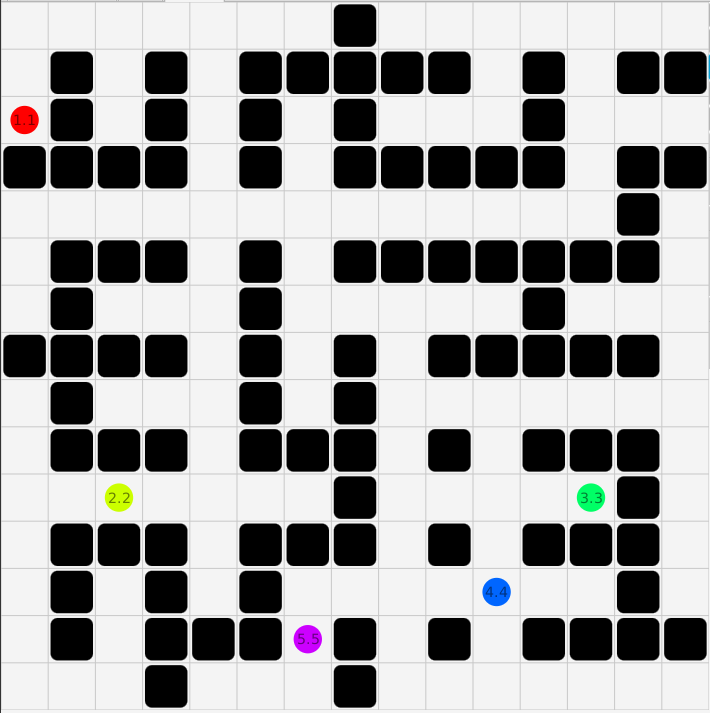
\includegraphics[width=0.6\columnwidth]{img/robopath/tests-15-15-5}
	\caption{Przykładowe środowisko typu M-15x15-5R - mapa $15 \times 15$ z wygenerowanym labiryntem, z 5 robotami w losowych położeniach}
	\label{fig:test-env-15-15-5}
\end{figure}
\begin{figure}
	\centering
	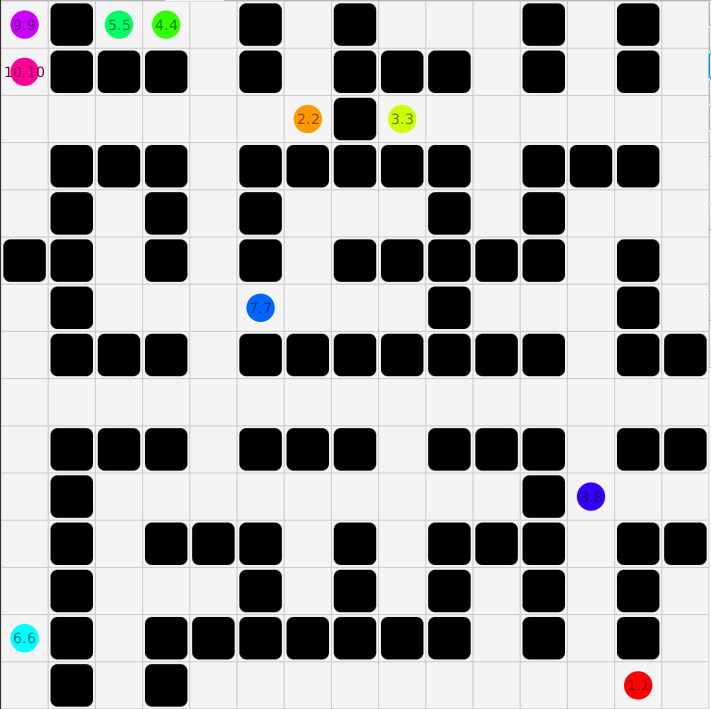
\includegraphics[width=0.6\columnwidth]{img/robopath/tests-15-15-10}
	\caption{Przykładowe środowisko typu M-15x15-10R - mapa $15 \times 15$ z wygenerowanym labiryntem, z 10 robotami w losowych położeniach}
	\label{fig:test-env-15-15-10}
\end{figure}
\begin{figure}
	\centering
	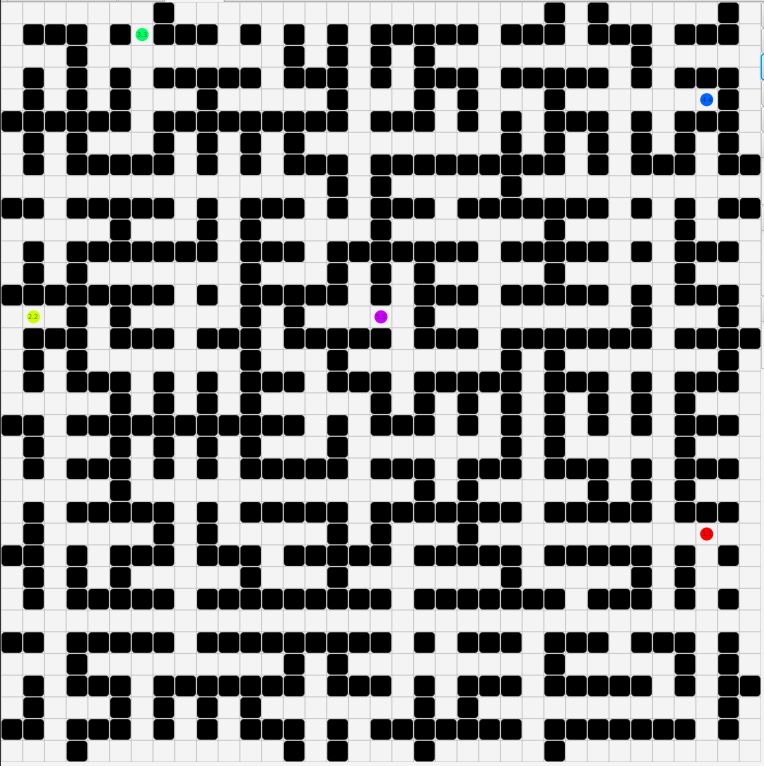
\includegraphics[width=0.6\columnwidth]{img/robopath/tests-35-35-5}
	\caption{Przykładowe środowisko typu M-35x35-5R - mapa $35 \times 35$ z wygenerowanym labiryntem, z 5 robotami w losowych położeniach}
	\label{fig:test-env-35-35-5}
\end{figure}
\begin{figure}
	\centering
	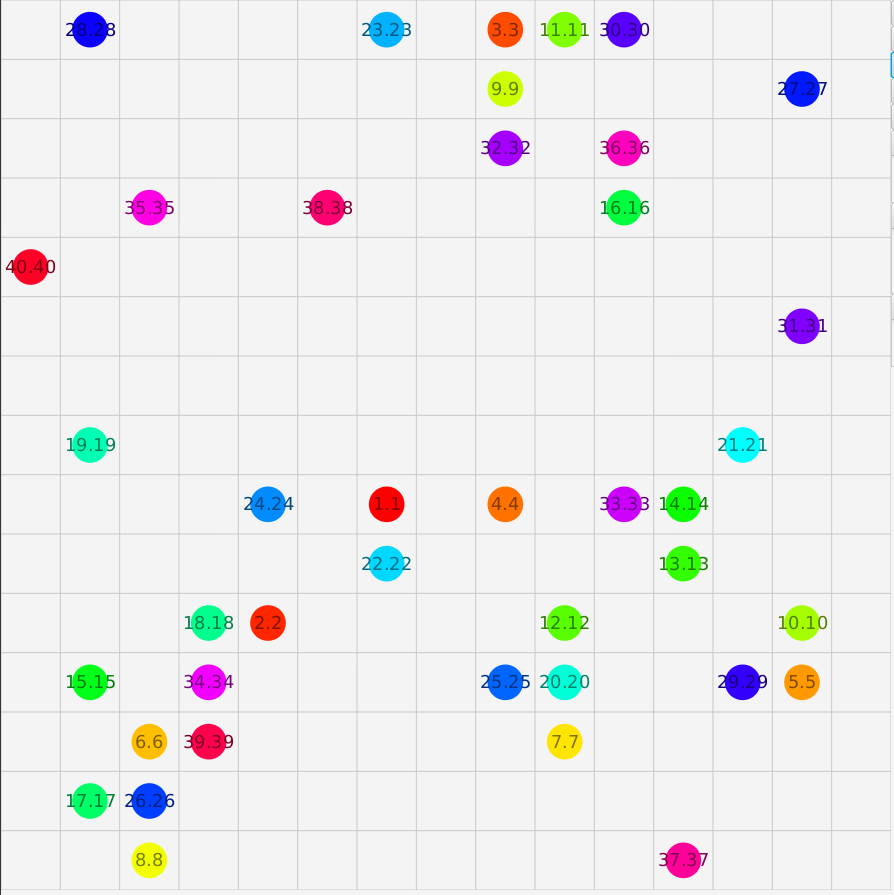
\includegraphics[width=0.6\columnwidth]{img/robopath/tests-15-15-empty-40}
	\caption{Przykładowe środowisko typu E-15x15-40R - mapa $15 \times 15$ bez przeszkód, z 40 robotami w losowych położeniach}
	\label{fig:test-env-15-15-empty-40}
\end{figure}

Dla każdego typu środowiska za każdym razem generowana jest nowa, losowa mapa. Również położenie początkowe i docelowe robotów jest losowane. Zatem w każdej symulacji wykorzystywane jest inne środowisko, chyba, że porównywane są między sobą różne metody. Wtedy rekonstruowane są te same warunki początkowe, aby przeprowadzić symulację ponownie z wykorzystaniem innej metody planowania.

Każdy z robotów otrzymuje losowe położenie początkowe. Jest to zawsze pole, na którym nie znajduje się przeszkoda, ani nie ma na nim innego robota.
Punkty docelowe także są losowane. Mogą to być pola, na których obecnie znajduje się jakiś robot, natomiast nie może to być punkt docelowy należący do innego robota, gdyż w przeciwnym wypadku uniemożliwiłoby to znalezienie rozwiązania, niezależnie od metody planowania.

\section{Wyniki testów}
\label{ch:test-results}
\subsection{Częstotliwość występowania potencjalnych kolizji} % 4000
Na początku przeprowadzamy testy częstotliwości występowania potencjalnych kolizji w badanych środowiskach, aby ocenić znaczenie tego problemu.
Dla każdego robota wykonujemy planowanie trasy za pomocą prostego algorytmu A*. Następnie przeprowadzamy symulację ruchu. W momencie wykrycia kolizji robotów zatrzymujemy symulację i zliczamy ilość takich sytuacji. W ten sposób mierzymy, jak często występują kolizję między robotami, jeśli planowanie odbywa się za pomocą algorytmu wyznaczania najkrótszych tras (bez unikania kolizji).
Słuszne jest założenie, że algorytm A* powinien zawsze znaleźć drogę do celu (z pominięciem pozostałych agentów), gdyż w tego typu środowiskach zawsze istnieje połączenie między dwoma dowolnymi polami na mapie \ref{ch:mazegen}.

W tabeli \ref{tab:test-collision-frequency} przedstawiono wyniki eksperymentów. Skuteczność oznacza w tym przypadku procentową liczbę symulacji, w których ruch wzdłuż zaplanowanych tras odbył się bez żadnych kolizji i wszystkie roboty zostały doprowadzone do celu.
Kolumna "Przeprowadzone symulacje" wyraża liczbę losowo wygenerowanych środowisk określonego typu.

\begin{table}[H]
\caption{Częstotliwość występowania kolizji w środowiskach zmierzona za pomocą skuteczności algorytmu A*}
\label{tab:test-collision-frequency}
\centering
\begin{tabular}{| l | r | r | r |}
\hline
\thead{\textbf{\shortstack{Typ\\środowiska}}} &
\thead{\textbf{\shortstack{Przeprowadzone\\symulacje}}} &
\thead{\textbf{\shortstack{Skuteczność}}} &
\thead{\textbf{\shortstack{Występowanie\\kolizji}}} \\ \hline
M-15x15-5R  & 1000 & 10\% & 90\% \\
M-15x15-10R & 1000 & 1\%  & 99\%  \\
M-35x35-5R  & 1000 & 14\% & 86\% \\
E-15x15-40R & 1000 & 0\%  & 100\%  \\ \hline
\end{tabular}
\end{table}

W tym teście przeprowadzono razem $4\ 000$ symulacji.

Uzyskane niskie wskaźniki skuteczności potwierdzają, że w tego typu środowiskach, problem występowania kolizji jest bardzo istotny i sam prosty algorytm A* nie wystarcza, aby poradzić sobie z bezkolizyjnym doprowadzeniem wszystkich robotów do celów.

\subsection{Wpływ wielkości okna czasowego} % 400
Zbadano skuteczność metody WHCA*1 (bez dynamicznego przydziału priorytetów) w zależności od wielkości okna czasowego, które to pozostaje stałe w trakcie trwania jednej symulacji.
Dla każdego badanego typu środowiska wylosowano 100 map, dla których powtórzono eksperymenty w tych samych warunkach, ale z różnymi rozmiarami okna czasowego od 1 do 30.
Dla rozmiaru okna równego 1 skuteczność metody zawsze jest zerowa, gdyż zaplanowane dla robotów ścieżki są zawsze długości 1, a pierwszym punktem ścieżki jest zawsze aktualna pozycja robota, przez co roboty pozostają w tym samym miejscu.
Uzyskane wyniki dla każdego środowiska przedstawiono w tabeli \ref{tab:test-whca-window-size} oraz na wykresach \ref{fig:test-whca-window-M-15x15-5R}, \ref{fig:test-whca-window-M-15x15-10R}, \ref{fig:test-whca-window-M-35x35-5R} i \ref{fig:test-whca-window-E-15x15-40R}.

{\renewcommand{\arraystretch}{0.9} % less cell spacing, default 1
\begin{table}[H]
\caption{Wpływ wielkości okna czasowego na skuteczność metody WHCA*1 w różnych typach środowisk} 
\label{tab:test-whca-window-size}
\centering
\small
\begin{tabular}{| r | r | r | r | r |}
\hline
\thead{\textbf{\shortstack{Rozmiar \\ okna \\ czasowego}}} &
\thead{\textbf{\shortstack{M-15x15-5R}}} &
\thead{\textbf{\shortstack{M-15x15-10R}}} &
\thead{\textbf{\shortstack{M-35x35-5R}}} &
\thead{\textbf{\shortstack{E-15x15-40R}}} \\ \hline
1	& 0\%	& 0\%	& 0\%	& 0\%	\\
2	& 9\%	& 0\%	& 27\%	& 0\%	\\
3	& 11\%	& 0\%	& 30\%	& 0\%	\\
4	& 11\%	& 0\%	& 43\%	& 0\%	\\
5	& 16\%	& 0\%	& 43\%	& 31\%	\\
6	& 21\%	& 0\%	& 48\%	& 65\%	\\
7	& 30\%	& 0\%	& 52\%	& 84\%	\\
8	& 35\%	& 5\%	& 61\%	& 93\%	\\
9	& 42\%	& 5\%	& 61\%	& 96\%	\\
10	& 42\%	& 7\%	& 61\%	& 98\%	\\
11	& 46\%	& 10\%	& 69\%	& 100\%	\\
12	& 53\%	& 12\%	& 74\%	& 100\%	\\
13	& 53\%	& 12\%	& 75\%	& 100\%	\\
14	& 61\%	& 12\%	& 75\%	& 100\%	\\
15	& 61\%	& 20\%	& 82\%	& 100\%	\\
16	& 62\%	& 20\%	& 82\%	& 100\%	\\
17	& 63\%	& 22\%	& 90\%	& 100\%	\\
18	& 64\%	& 23\%	& 90\%	& 100\%	\\
19	& 64\%	& 23\%	& 92\%	& 100\%	\\
20	& 65\%	& 26\%	& 95\%	& 100\%	\\
21	& 65\%	& 26\%	& 100\%	& 100\%	\\
22	& 65\%	& 26\%	& 100\%	& 100\%	\\
23	& 67\%	& 30\%	& 100\%	& 100\%	\\
24	& 67\%	& 33\%	& 100\%	& 100\%	\\
25	& 67\%	& 33\%	& 100\%	& 100\%	\\
26	& 69\%	& 33\%	& 100\%	& 100\%	\\
27	& 69\%	& 33\%	& 100\%	& 100\%	\\
28	& 69\%	& 35\%	& 100\%	& 100\%	\\
29	& 69\%	& 35\%	& 100\%	& 100\%	\\
30	& 69\%	& 35\%	& 100\%	& 100\%	\\
\hline
\end{tabular}
\end{table}}

\begin{figure}
	\centering
	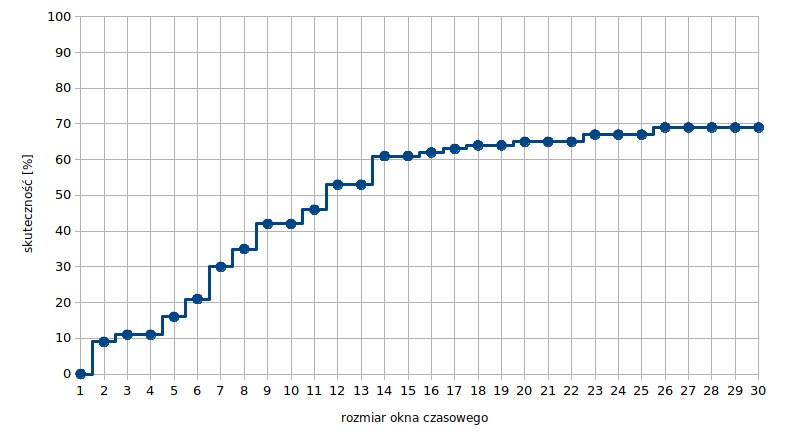
\includegraphics[width=0.8\columnwidth]{img/plots/test-whca-window-M-15x15-5R}
	\caption{Wykres skuteczności metody WHCA* w zależności od rozmiaru okna czasowego dla środowiska typu M-15x15-5R}
	\label{fig:test-whca-window-M-15x15-5R}
\end{figure}
\begin{figure}
	\centering
	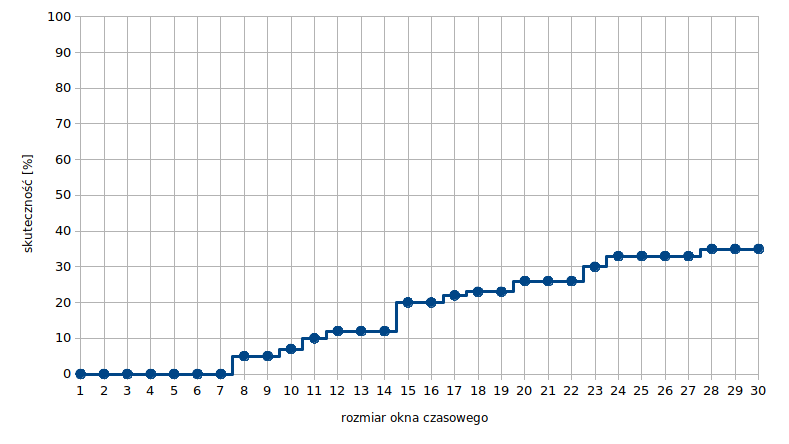
\includegraphics[width=0.8\columnwidth]{img/plots/test-whca-window-M-15x15-10R}
	\caption{Wykres skuteczności metody WHCA* w zależności od rozmiaru okna czasowego dla środowiska typu M-15x15-10R}
	\label{fig:test-whca-window-M-15x15-10R}
\end{figure}
\begin{figure}
	\centering
	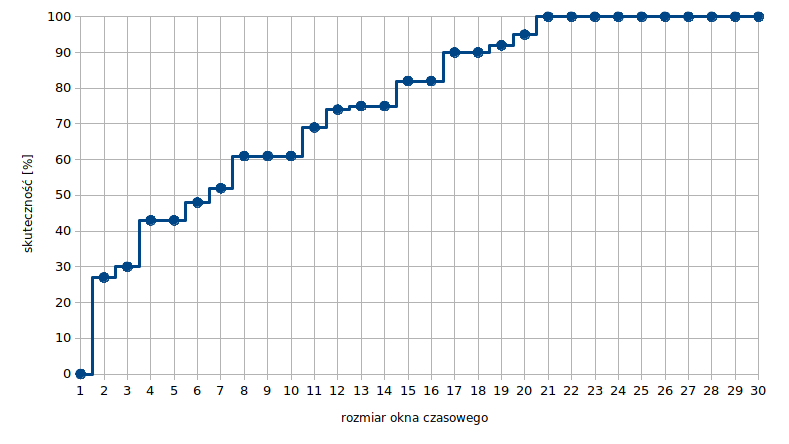
\includegraphics[width=0.8\columnwidth]{img/plots/test-whca-window-M-35x35-5R}
	\caption{Wykres skuteczności metody WHCA* w zależności od rozmiaru okna czasowego dla środowiska typu M-35x35-5R}
	\label{fig:test-whca-window-M-35x35-5R}
\end{figure}
\begin{figure}
	\centering
	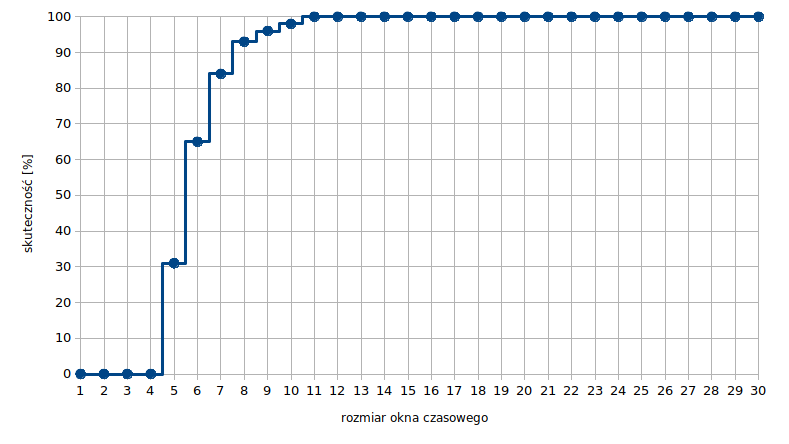
\includegraphics[width=0.8\columnwidth]{img/plots/test-whca-window-E-15x15-40R}
	\caption{Wykres skuteczności metody WHCA* w zależności od rozmiaru okna czasowego dla środowiska typu E-15x15-40R}
	\label{fig:test-whca-window-E-15x15-40R}
\end{figure}

W tych testach przeprowadzono razem $400$ symulacji.

Zgodnie z oczekiwaniami skuteczność metody WHCA*1 rośnie monotonicznie wraz ze wzrostem rozmiaru okna czasowego.

\subsection{Skuteczność LRA* i WHCA*3} %8000
W następnym eksperymencie przeprowadzono serie testów mających na celu porównanie skuteczności metody LRA* oraz WHCA*3 z dynamicznym przydziałem priorytetów.
Mapy generowane były losowo, natomiast dla każdego środowiska symulacja została wykonana dwukrotnie: raz wykonując planowanie tras metodą WHCA*3 a następnie metodą LRA* po odtworzeniu tych samych warunków początkowych.
Dla każdej takiej symulacji zliczano, ile razy obie metody pomyślnie doprowadziły wszystkie roboty do celu ("Sukces WHCA*3 i LRA*"), ile razy powiodła się tylko metoda WHCA*3 ("Sukces tylko WHCA*3"), ile razy tylko metoda LRA* ("Sukces tylko LRA*"), oraz ile razy żadna z metod nie zakończyła się powodzeniem ("Brak sukcesu").
Umożliwiło to porównanie skuteczności metod w dokładnie tych samym warunkach. Wyniki przedstawiono w tabeli \ref{tab:test-lra-whca-effectiveness}.
Dla każdego typu środowiska wygenerowano 1000 map z różnymi układami robotów.
W ramach tych testów przeprowadzono razem $8\ 000$ symulacji.

\begin{table}[H]
\caption{Porównanie skuteczności LRA* i WHCA*3 w tych samych warunkach}
\label{tab:test-lra-whca-effectiveness}
\centering
\begin{tabular}{| l | r | r | r | r | r |}
\hline
\thead{\textbf{\shortstack{Typ\\środowiska}}} &
\thead{\textbf{\shortstack{Sukces\\WHCA*3\\i LRA*}}} &
\thead{\textbf{\shortstack{Sukces\\tylko\\WHCA*3}}} &
\thead{\textbf{\shortstack{Sukces\\tylko\\LRA*}}} &
\thead{\textbf{\shortstack{Brak\\sukcesu}}} \\ \hline
M-15x15-5R  & 23,0\% & 66,7\% & 0\% & 10,3\% \\ 
M-15x15-10R & 1,2\%  & 64,0\% & 0\% & 34,8\% \\ 
M-35x35-5R  & 51,3\% & 47,1\% & 0\% & 1,6\%  \\ 
E-15x15-40R & 82,3\% & 17,7\% & 0\% & 0\%    \\ \hline
\end{tabular}
\end{table}

Warto zaznaczyć, że niepowodzenie metody WHCA*3 może wynikać zarówno z ograniczeń metody, jak i z przypadkowego wylosowania układu przeszkód i robotów, który sam w sobie jest niemożliwy do rozwiązania.
Należy także podkreślić, że spośród wszystkich środowisk nie zdarzyło się, aby metoda LRA* powiodła się, podczas gdy WHCA*3 nie znalazła rozwiązania.
Potwierdza to oczekiwania w stosunku do metody WHCA*3, która jest znacznie bardziej zaawansowana od metody LRA*.

\subsection{Porównanie wariantów WHCA*} % 16000
W kolejnych testach porównano skuteczność różnych wariantów metody WHCA*: WHCA*1, WHCA*2 (z dynamicznym przydziałem priorytetów), WHCA*3 (z dynamicznym przydziałem priorytetów i skalowaniem okna czasowego) oraz metodę LRA*.
Symulacje powtarzano dla każdej metody, odtwarzając te same warunki początkowe (układ map, robotów i punktów docelowych).
Wyniki przedstawiono w tabeli \ref{tab:test-lra-whca-whca2-effectiveness}.
Dla każdego typu środowiska wygenerowano 1000 map z różnymi układami robotów.
W ramach tych testów przeprowadzono razem $16\ 000$ symulacji.

\begin{table}[H]
\caption{Porównanie skuteczności metod LRA*, WHCA*1, WHCA*2, WHCA*3}
\label{tab:test-lra-whca-whca2-effectiveness}
\centering
\begin{tabular}{| l | r | r | r | r | r |}
\hline
\thead{\textbf{\shortstack{Typ\\środowiska}}} &
\thead{\textbf{\shortstack{Skuteczność\\LRA*}}} &
\thead{\textbf{\shortstack{Skuteczność\\WHCA*1}}} &
\thead{\textbf{\shortstack{Skuteczność\\WHCA*2}}} &
\thead{\textbf{\shortstack{Skuteczność\\WHCA*3}}} \\ \hline
M-15x15-5R  & 22,5\% & 26,3\%  & 54,6\% & 87\%   \\ 
M-15x15-10R & 0,2\%  & 3,4\%   & 48,9\% & 54,5\% \\ 
M-35x35-5R  & 52,7\% & 40,1\%  & 69,7\% & 98,6\% \\ 
E-15x15-40R & 76,7\% & 99,5\%  & 100\%  & 100\%  \\ \hline
\end{tabular}
\end{table}

Wyniki potwierdzają oczekiwaną nierówność zachodzącą pomiędzy średnimi skutecznościami poszczególnych metod dla każdego z badanych typów środowisk.
% skuteczność LRA* $\le$ skuteczność WHCA*1 $\le$ skuteczność WHCA*2 $\le$ skuteczność WHCA*3.
% Warto dodać, że w pewnych sytuacjach algorytm LRA* pomyślnie doprowadził wszystkie roboty do ich celów, podczas gdy w tych samych warunkach metody WHCA*1 i WHCA*2 nie znalazły rozwiązania.

\subsection{Wpływ rozmiaru mapy} % 24400 = 15200 + 9200
\label{ch:tests-function-mapsize}
Dla stałej liczby robotów (równej 5) przeprowadzono testy wpływu rozmiaru mapy na skuteczność metod LRA*, WHCA*1, WHCA*2 oraz WHCA*3.
Dla każdej z metod zmierzono także średnią liczbę kroków symulacji potrzebną do doprowadzenia wszystkich robotów do celów (dla symulacji zakończonych powodzeniem) oraz złożoność obliczeniową samego planowania (średni czas wykonywania obliczeń dla wyznaczania tras w ciągu całej symulacji).
Symulacje przeprowadzano na kwadratowych mapach.
Rozmiar mapy zmieniał się w zakresie od $3 \times 3$ do $40 \times 40$ (w przypadku mapy z labiryntem) oraz w zakresie od $3 \times 3$ do $25 \times 25$ (w przypadku pustej mapy), generując 100 losowych układów dla każdego rozmiaru mapy, następnie dla każdego takiego układu wykonano symulację każdą z 4 badanych metod.
Wszystko powtórzono zarówno dla map z wygenerowanym labiryntem, jak i dla pustych map bez umieszczonych przeszkód.

W ramach tych testów przeprowadzono razem $24\ 400$ symulacji.
Wyniki przedstawiono na wykresach \ref{fig:test-steps-maze-mapsize-eff}, \ref{fig:test-steps-maze-mapsize-steps}, \ref{fig:test-steps-maze-mapsize-calctime}, \ref{fig:test-steps-empty-mapsize-eff}, \ref{fig:test-steps-empty-mapsize-steps}, \ref{fig:test-steps-empty-mapsize-calctime}.

% w tabelach \ref{tab:test-steps-maze-mapsize}, \ref{tab:test-steps-empty-mapsize} oraz
% $TODO$ zrobić tabelki (screeny) i wykresy

% \begin{table}
% \caption{Wskaźniki symulacji dla metod LRA*, WHCA*1, WHCA*2 i WHCA*3 w zależności od rozmiaru mapy, z wygenerowanym labiryntem}
% \label{tab:test-steps-maze-mapsize}
% \centering
% \begin{tabular}{| r | r | r | r | r | r | r | r | r | r | r | r | r |}
% \hline
% {\bf \shortstack{Rozmiar\\mapy}} &
% {\bf \shortstack{Skuteczność\\LRA*}} &
% {\bf \shortstack{Skuteczność\\WHCA*1}} &
% {\bf \shortstack{Skuteczność\\WHCA*2}} &
% {\bf \shortstack{Skuteczność\\WHCA*3}} &
% {\bf \shortstack{Liczba kroków\\LRA*}} &
% {\bf \shortstack{Liczba kroków\\WHCA*1}} &
% {\bf \shortstack{Liczba kroków\\WHCA*2}} &
% {\bf \shortstack{Liczba kroków\\WHCA*3}} &
% {\bf \shortstack{Czas planowania\\LRA*}} &
% {\bf \shortstack{Czas planowania\\WHCA*1}} &
% {\bf \shortstack{Czas planowania\\WHCA*2}} &
% {\bf \shortstack{Czas planowania\\WHCA*3}} \\ \hline
% 1 &  &  &  &  &  &  &  &  &  &  &  &  \\ \hline
% \end{tabular}
% \end{table}
% \begin{table}
% \caption{Wskaźniki symulacji dla metod LRA*, WHCA*1, WHCA*2 i WHCA*3 w zależności od rozmiaru mapy, bez umieszczonych przeszkód}
% \label{tab:test-steps-empty-mapsize}
% \centering
% \begin{tabular}{| r | r | r | r | r | r | r | r | r | r | r | r | r |}
% \hline
% {\bf \shortstack{Rozmiar\\mapy}} &
% {\bf \shortstack{Skuteczność\\LRA*}} &
% {\bf \shortstack{Skuteczność\\WHCA*1}} &
% {\bf \shortstack{Skuteczność\\WHCA*2}} &
% {\bf \shortstack{Skuteczność\\WHCA*3}} &
% {\bf \shortstack{Liczba kroków\\LRA*}} &
% {\bf \shortstack{Liczba kroków\\WHCA*1}} &
% {\bf \shortstack{Liczba kroków\\WHCA*2}} &
% {\bf \shortstack{Liczba kroków\\WHCA*3}} &
% {\bf \shortstack{Czas planowania\\LRA*}} &
% {\bf \shortstack{Czas planowania\\WHCA*1}} &
% {\bf \shortstack{Czas planowania\\WHCA*2}} &
% {\bf \shortstack{Czas planowania\\WHCA*3}} \\ \hline
% 1 &  &  &  &  &  &  &  &  &  &  &  &  \\ \hline
% \end{tabular}
% \end{table}

\begin{figure}[H]
	\centering
	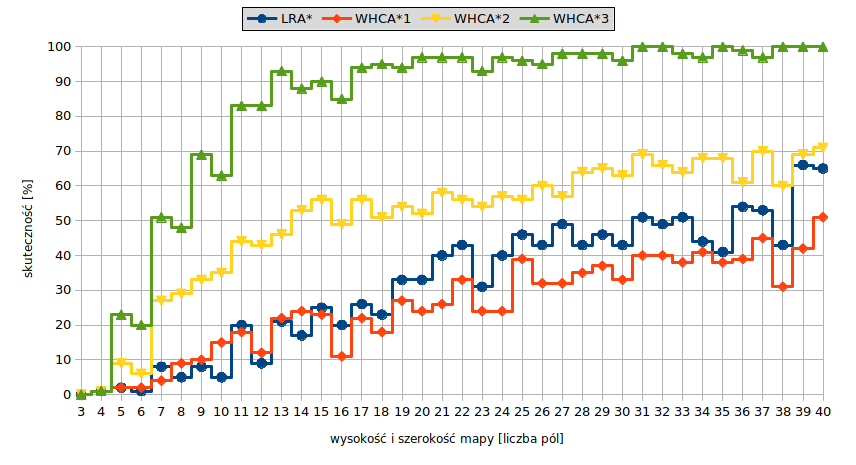
\includegraphics[width=0.9\columnwidth]{img/plots/test-steps-maze-mapsize-eff}
	\caption{Wykres skuteczności metod LRA*, WHCA*1, WHCA*2 i WHCA*3 w zależności od rozmiaru mapy, z wygenerowanym labiryntem}
	\label{fig:test-steps-maze-mapsize-eff}
\end{figure}
\begin{figure}[H]
	\centering
	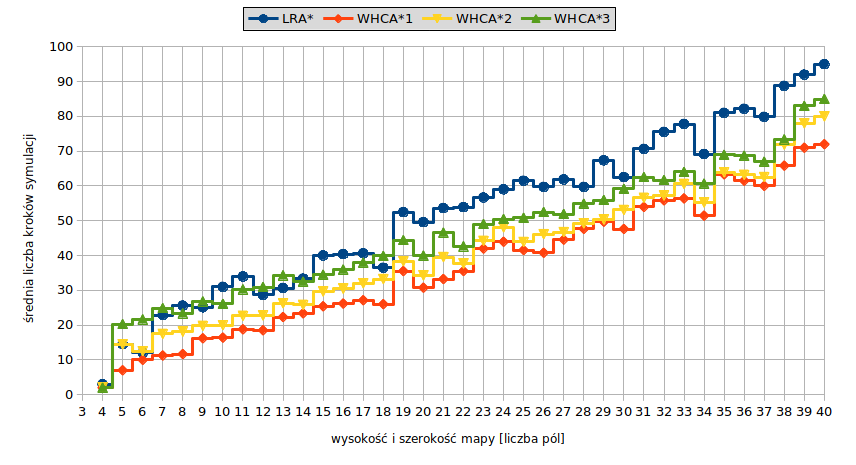
\includegraphics[width=0.9\columnwidth]{img/plots/test-steps-maze-mapsize-steps}
	\caption{Wykres średniej liczby kroków symulacji dla metod LRA*, WHCA*1, WHCA*2 i WHCA*3 w zależności od rozmiaru mapy, z wygenerowanym labiryntem}
	\label{fig:test-steps-maze-mapsize-steps}
\end{figure}
\begin{figure}[H]
	\centering
	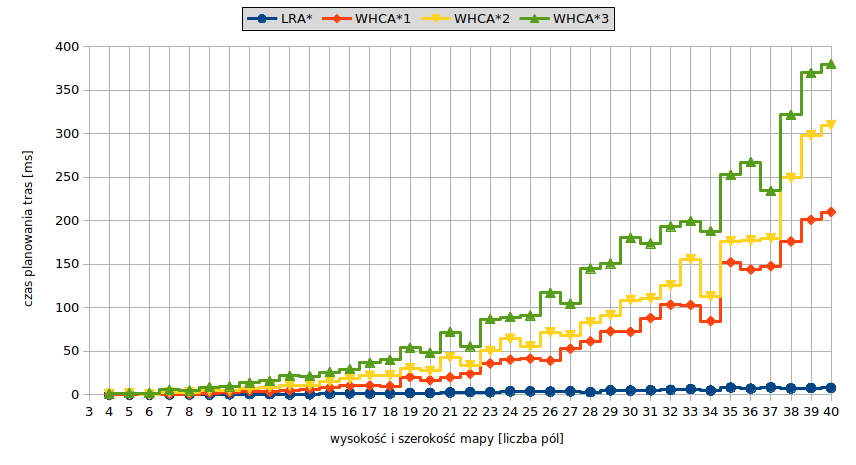
\includegraphics[width=0.9\columnwidth]{img/plots/test-steps-maze-mapsize-calctime}
	\caption{Wykres czasu planowania dla metod LRA*, WHCA*1, WHCA*2 i WHCA*3 w zależności od rozmiaru mapy, z wygenerowanym labiryntem}
	\label{fig:test-steps-maze-mapsize-calctime}
\end{figure}
\begin{figure}[H]
	\centering
	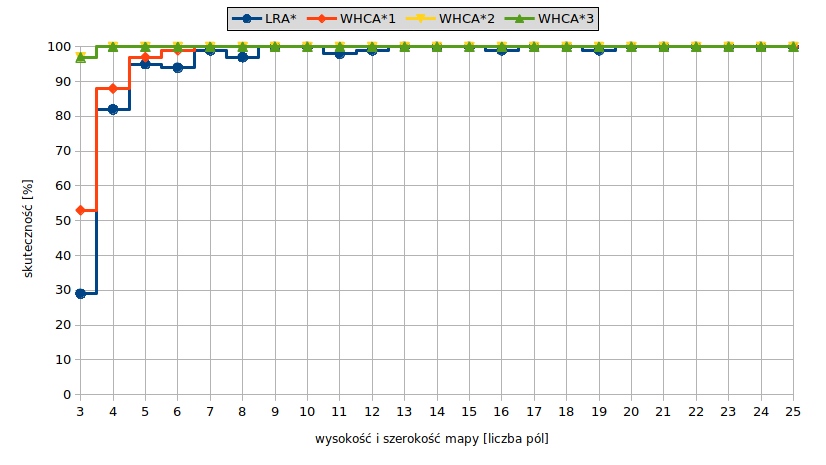
\includegraphics[width=0.9\columnwidth]{img/plots/test-steps-empty-mapsize-eff}
	\caption{Wykres skuteczności metod LRA*, WHCA*1, WHCA*2 i WHCA*3 w zależności od rozmiaru mapy, bez przeszkód na mapie (wykresy WHCA*1, WHCA*2, WHCA*3 prawie pokrywają się)}
	\label{fig:test-steps-empty-mapsize-eff}
\end{figure}
\begin{figure}[H]
	\centering
	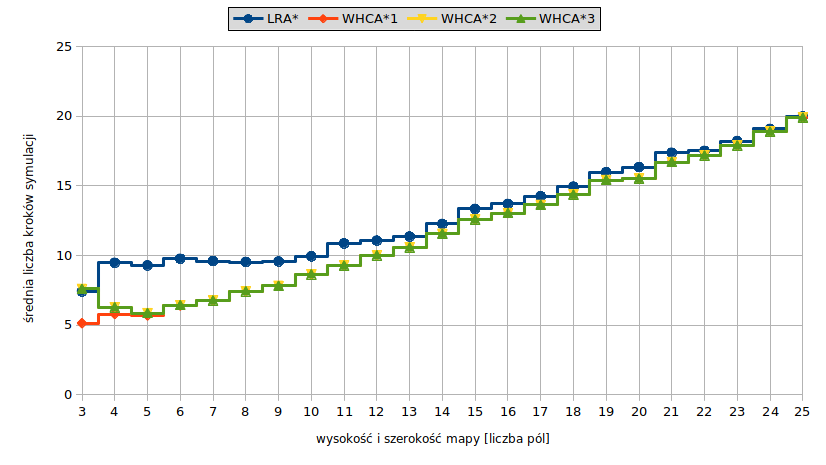
\includegraphics[width=0.9\columnwidth]{img/plots/test-steps-empty-mapsize-steps}
	\caption{Wykres średniej liczby kroków symulacji dla metod LRA*, WHCA*1, WHCA*2 i WHCA*3 w zależności od rozmiaru mapy, bez przeszkód na mapie}
	\label{fig:test-steps-empty-mapsize-steps}
\end{figure}
\begin{figure}[H]
	\centering
	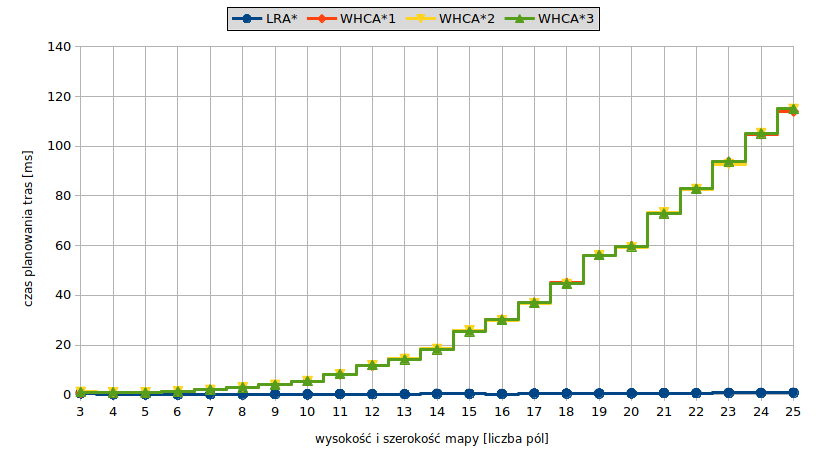
\includegraphics[width=0.9\columnwidth]{img/plots/test-steps-empty-mapsize-calctime}
	\caption{Wykres czasu planowania dla metod LRA*, WHCA*1, WHCA*2 i WHCA*3 w zależności od rozmiaru mapy, bez przeszkód na mapie}
	\label{fig:test-steps-empty-mapsize-calctime}
\end{figure}


\subsection{Wpływ liczby robotów} % 24000
\label{ch:tests-function-robots}
Dla stałego rozmiaru mapy przeprowadzono testy wpływu liczby robotów na skuteczność metod LRA*, WHCA*1, WHCA*2 oraz WHCA*3.
Dla każdej z metod zmierzono także średnią liczbę kroków symulacji potrzebną do doprowadzenia wszystkich robotów do celów (dla symulacji zakończonych powodzeniem) oraz złożoność obliczeniową samego planowania (średni czas wykonywania obliczeń dla wyznaczania tras w ciągu całej symulacji).
Liczbę robotów zwiększano od $1$ do $30$, generując 100 losowych układów dla każdej liczby robotów, następnie dla każdego takiego układu wykonano symulację każdą z 4 badanych metod.
Wszystko powtórzono zarówno dla map z wygenerowanym labiryntem o rozmiarze $15 \times 15$, jak i dla pustych map bez umieszczonych przeszkód o rozmiarze $6 \times 6$.

W ramach tych testów przeprowadzono razem $24\ 000$ symulacji.
Wyniki przedstawiono na wykresach \ref{fig:test-steps-maze-robots-eff}, \ref{fig:test-steps-maze-robots-steps}, \ref{fig:test-steps-maze-robots-calctime}, \ref{fig:test-steps-empty-robots-eff}, \ref{fig:test-steps-empty-robots-steps}, \ref{fig:test-steps-empty-robots-calctime}.

% w tabelach \ref{tab:test-steps-maze-robots}, \ref{tab:test-steps-empty-robots} oraz
% $TODO$ zrobić tabelki (screeny) i wykresy

% \begin{table}
% \caption{Wskaźniki symulacji dla metod LRA*, WHCA*1, WHCA*2 i WHCA*3 w zależności od liczby robotów, z wygenerowanym labiryntem}
% \label{tab:test-steps-maze-robots}
% \centering
% \begin{tabular}{| r | r | r | r | r | r | r | r | r | r | r | r | r |}
% \hline
% {\bf \shortstack{Liczba\\robotów}} &
% {\bf \shortstack{Skuteczność\\LRA*}} &
% {\bf \shortstack{Skuteczność\\WHCA*1}} &
% {\bf \shortstack{Skuteczność\\WHCA*2}} &
% {\bf \shortstack{Skuteczność\\WHCA*3}} &
% {\bf \shortstack{Liczba kroków\\LRA*}} &
% {\bf \shortstack{Liczba kroków\\WHCA*1}} &
% {\bf \shortstack{Liczba kroków\\WHCA*2}} &
% {\bf \shortstack{Liczba kroków\\WHCA*3}} &
% {\bf \shortstack{Czas planowania\\LRA*}} &
% {\bf \shortstack{Czas planowania\\WHCA*1}} &
% {\bf \shortstack{Czas planowania\\WHCA*2}} &
% {\bf \shortstack{Czas planowania\\WHCA*3}} \\ \hline
% 1 &  &  &  &  &  &  &  &  &  &  &  &  \\ \hline
% \end{tabular}
% \end{table}
% \begin{table}
% \caption{Wskaźniki symulacji dla metod LRA*, WHCA*1, WHCA*2 i WHCA*3 w zależności od liczby robotów, bez umieszczonych przeszkód}
% \label{tab:test-steps-empty-robots}
% \centering
% \begin{tabular}{| r | r | r | r | r | r | r | r | r | r | r | r | r |}
% \hline
% {\bf \shortstack{Liczba\\robotów}} &
% {\bf \shortstack{Skuteczność\\LRA*}} &
% {\bf \shortstack{Skuteczność\\WHCA*1}} &
% {\bf \shortstack{Skuteczność\\WHCA*2}} &
% {\bf \shortstack{Skuteczność\\WHCA*3}} &
% {\bf \shortstack{Liczba kroków\\LRA*}} &
% {\bf \shortstack{Liczba kroków\\WHCA*1}} &
% {\bf \shortstack{Liczba kroków\\WHCA*2}} &
% {\bf \shortstack{Liczba kroków\\WHCA*3}} &
% {\bf \shortstack{Czas planowania\\LRA*}} &
% {\bf \shortstack{Czas planowania\\WHCA*1}} &
% {\bf \shortstack{Czas planowania\\WHCA*2}} &
% {\bf \shortstack{Czas planowania\\WHCA*3}} \\ \hline
% 1 &  &  &  &  &  &  &  &  &  &  &  &  \\ \hline
% \end{tabular}
% \end{table}

\begin{figure}[H]
	\centering
	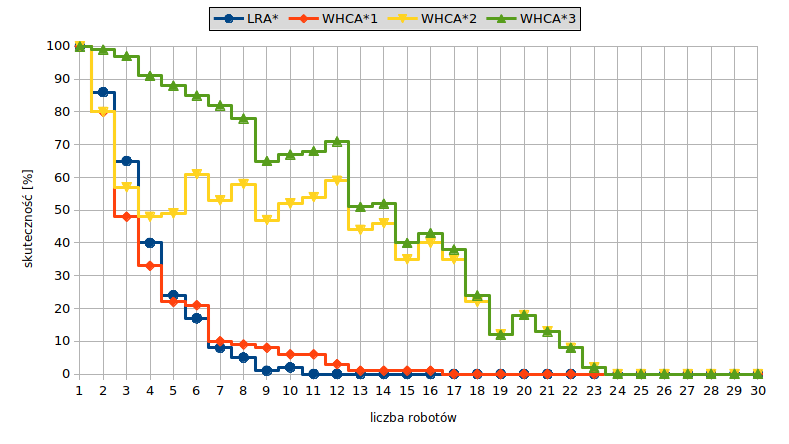
\includegraphics[width=0.9\columnwidth]{img/plots/test-steps-maze-robots-eff}
	\caption{Wykres skuteczności metod LRA*, WHCA*1, WHCA*2 i WHCA*3 w zależności od liczby robotów, z wygenerowanym labiryntem}
	\label{fig:test-steps-maze-robots-eff}
\end{figure}
\begin{figure}[H]
	\centering
	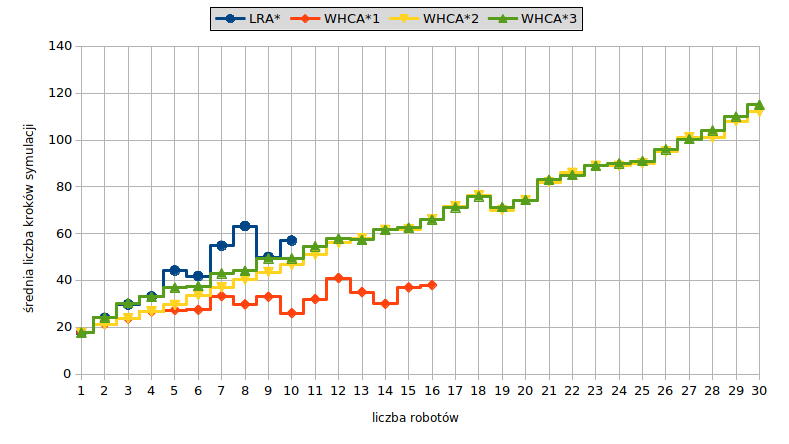
\includegraphics[width=0.9\columnwidth]{img/plots/test-steps-maze-robots-steps}
	\caption{Wykres średniej liczby kroków symulacji dla metod LRA*, WHCA*1, WHCA*2 i WHCA*3 w zależności od liczby robotów, z wygenerowanym labiryntem}
	\label{fig:test-steps-maze-robots-steps}
\end{figure}
\begin{figure}[H]
	\centering
	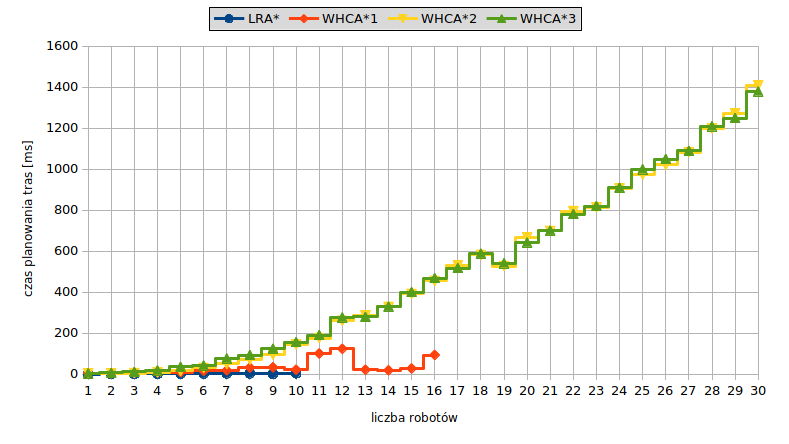
\includegraphics[width=0.9\columnwidth]{img/plots/test-steps-maze-robots-calctime}
	\caption{Wykres czasu planowania dla metod LRA*, WHCA*1, WHCA*2 i WHCA*3 w zależności od liczby robotów, z wygenerowanym labiryntem}
	\label{fig:test-steps-maze-robots-calctime}
\end{figure}
\begin{figure}[H]
	\centering
	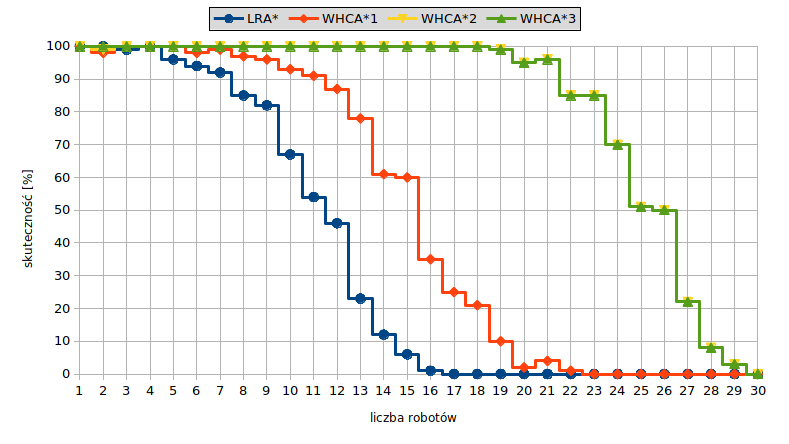
\includegraphics[width=0.9\columnwidth]{img/plots/test-steps-empty-robots-eff}
	\caption{Wykres skuteczności metod LRA*, WHCA*1, WHCA*2 i WHCA*3 w zależności od liczby robotów, bez przeszkód na mapie}
	\label{fig:test-steps-empty-robots-eff}
\end{figure}
\begin{figure}[H]
	\centering
	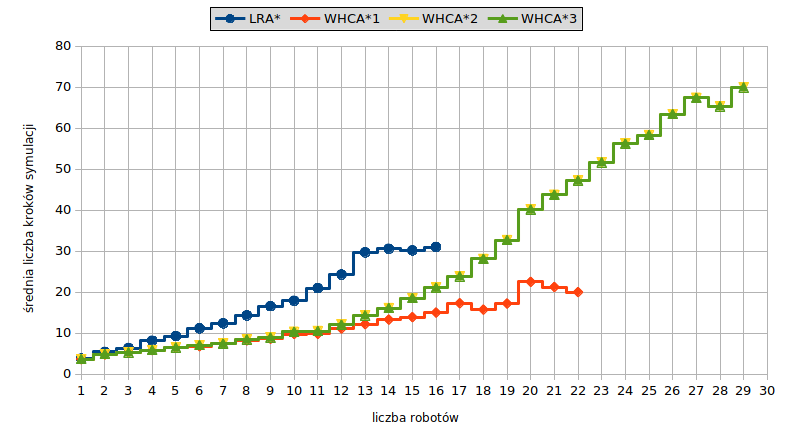
\includegraphics[width=0.9\columnwidth]{img/plots/test-steps-empty-robots-steps}
	\caption{Wykres średniej liczby kroków symulacji dla metod LRA*, WHCA*1, WHCA*2 i WHCA*3 w zależności od liczby robotów, bez przeszkód na mapie}
	\label{fig:test-steps-empty-robots-steps}
\end{figure}
\begin{figure}[H]
	\centering
	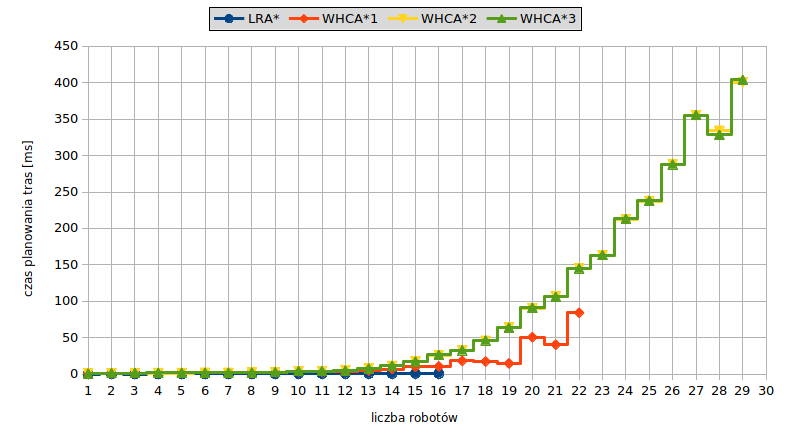
\includegraphics[width=0.9\columnwidth]{img/plots/test-steps-empty-robots-calctime}
	\caption{Wykres czasu planowania dla metod LRA*, WHCA*1, WHCA*2 i WHCA*3 w zależności od liczby robotów, bez przeszkód na mapie}
	\label{fig:test-steps-empty-robots-calctime}
\end{figure}

Na wykresach średniej liczby kroków symulacji oraz czasu planowania widoczne są "ucięte" serie pomiarów. Oznacza to zerową skuteczność w tych obszarach i tym samym brak możliwości wyznaczenia tych wartości z powodu zerowej liczby pomyślnie zakończonych symulacji dla danej metody planowania.

% Wyniki potwierdzają oczekiwaną nierówność zachodzącą pomiędzy średnimi skutecznościami poszczególnych metod dla każdego z badanych typów środowisk:
% skuteczność WHCA*1 $\le$ skuteczność WHCA*2 $\le$ skuteczność WHCA*3.
Zgodny z oczekiwaniami jest niewątpliwy fakt, iż zwiększenie liczby robotów utrudnia znalezienie rozwiązania, zmniejszając skuteczność metod.
% Na pustych mapach bez przeszkód metody WHCA*2 i WHCA*3 mają wysoką skuteczność, ale ilość kroków symulacji potrzebnych do znalezienia rozwiązania jest większa niż dla metody WHCA*1.

\subsection{Metoda pól potencjałowych}
Metoda pól potencjałowych zaimplementowana w aplikacji okazała się mieć bardzo niską skuteczność w doprowadzeniu do celu nawet jednego robota.
Tym bardziej nie nadaje się do skutecznego rozwiązania skomplikowanego zagadnienia znalezienia bezkolizyjnych tras dla wielu robotów.
Niska skuteczność metody wynika m.in. z charakteru wygenerowanych map, w których robot bardzo często napotyka na lokalne minimum, z którego nie potrafi się wydostać.
Przykład uwięzienia robota w takiej "studni potencjału" został przedstawiony na rysunku \ref{fig:test-field-potential-hole}.

\begin{figure}[H]
	\centering
	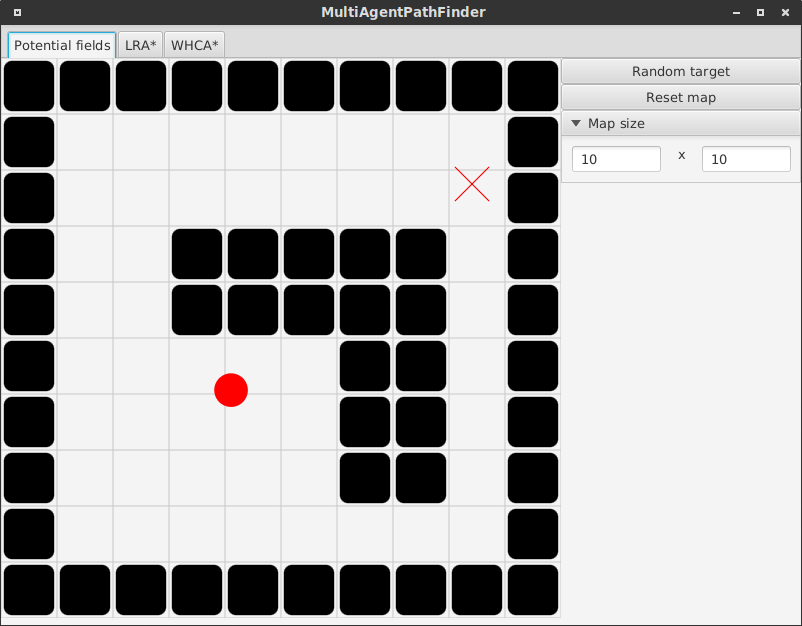
\includegraphics[width=0.6\columnwidth]{img/robopath/field-potential-hole}
	\caption{Robot prowadzony metodą pól potencjałowych uwięziony w studni potencjału. Zerowa siła wypadkowa nie pozwala mu dotrzeć do celu.}
	\label{fig:test-field-potential-hole}
\end{figure}

\section{Dyskusja wyników}
Przeprowadzenie eksperymentów, które pozwoliłyby uzyskać niepodważalne wnioski, jest bardzo trudnym zadaniem w przypadku metod planowania tras.
Należy pamiętać, że porównanie wyników badanych algorytmów możliwe jest jedynie w kontekście indywidualnej, pojedynczej konfiguracji przeszkód i robotów na mapie.
Zatem utrudnione jest otrzymanie ogólnego wniosku, który byłby prawdziwy dla wszystkich możliwych układów robotów.
Z tego powodu testy zostały przeprowadzone w dużej ilości, w losowych środowiskach, a następnie posłużono się statystyką w celu generalizacji uzyskanych rezultatów.

Warto zaznaczyć, że nie dysponujemy zupełną metodą planowania tras, która byłaby w stanie znaleźć zawsze optymalne rozwiązanie lub obiektywnie stwierdzić, że żadne rozwiązanie nie istnieje.
Niestety brak takiego źródła referencyjnego nie pozwala w pełni ocenić skuteczności badanych metod. W szczególności nie można stwierdzić, czy testowana metoda planowania nie uzyskała rozwiązania z powodu własnych ograniczeń, czy też z powodu tego, że wylosowany układ przeszkód i robotów był sam w sobie niemożliwy do rozwiązania.
Możliwe natomiast jest porównanie rezultatów różnych metod planowania w tych samych warunkach początkowych, co może dostarczyć pewnych wniosków.

Należy pamiętać, że ze względu na wybraną technologię realizacji (Java), pomiar czasu obliczeń mógł być obarczony pewnymi błędami wynikającymi z narzutu wirtualnej maszyny JVM oraz działania mechanizmu zwalniania pamięci przez Garbage Collector, co wstrzymuje aplikację na pewien czas.
Na takie zdarzenie nie ma wpływu programista, a może ono wystąpić w dowolnym momencie działania aplikacji, powodując przekłamania zmierzonego czasu.

Wyniki testów potwierdziły oczekiwania w stosunku do skuteczności porównywanych metod.
Najwyższą skuteczność w planowaniu bezkolizyjnych tras dla wielu robotów uzyskała autorska metoda WHCA*3.
Brak zastosowania skalowania okna czasowego skutkował niższą skutecznością metody WHCA*2.
W badanych środowiskach najgorzej wypadły metody LRA* oraz WHCA*1.
% $TODO$ bez dyhnamicznego przydziału priorytetów - gorzej WHCA*1
% $TODO$ najgorzej lra

% LRA: wyszło całkiem nieźle w przypadku, gdy do celu prowadzi wiele alternatywnych ścieżek i można ominąć wąskie gardło
% potwierdzenie oczekiwań (poprawności) - nigdy nie było tak, żeby LRA był lepszy

Na dużych mapach oraz przy większej liczbie robotów czas wykonywania obliczeń planowania tras przez metodę WHCA*3 jest stosunkowo długi.
Obserwacja czasu obliczeń pozwala stwierdzić, że złożoność WHCA*3 ma charakter wykładniczy, co także potwierdza oczekiwania.
Zastosowanie do wyznaczania wartości heurystyki innych, wydajniejszych algorytmów takich jak RRA*, D* Lite lub D* Extra Lite, mogłoby zmniejszyć czas obliczeń, przyspieszając proces planowania bezkolizyjnych tras, w szczególności na większych mapach.

% TODO przykład rozwiązania deadlocka w kilku screenach
% autorski WHCA*3 działa dobrze nawet przy rozwiązywaniu dużych deadlocków

% $TODO$ wnioski o zachodzących nierównościach
